% ============================================================
% main.tex
% bipolar SPWM + V/f Control for Variable Frequency Drives
% Reviewer-independent, RTL-credible, compile-clean
% ============================================================

\documentclass[12pt]{article}

\usepackage[margin=1in]{geometry}
\usepackage{amsmath, amssymb, amsfonts}
\usepackage{booktabs}
\usepackage{siunitx}
\usepackage{graphicx}
\usepackage{subcaption}
\usepackage{hyperref}
\usepackage{float}
\usepackage{xcolor}
\usepackage{array}
\usepackage{grffile}   % robust filename handling
\usepackage{ifthen}

% TikZ for architecture, FSM, and circuit sketches
\usepackage{tikz}
\usetikzlibrary{arrows.meta, positioning, shapes.geometric, automata}

\hypersetup{
  colorlinks=true,
  linkcolor=blue,
  urlcolor=blue,
  citecolor=blue
}

% Graphics search paths
\graphicspath{{../out/report/}{../out/report/analysis/}{../out/report/sweep/}{../out/report/sweep/waves/}}

\title{Bipolar Sinusoidal PWM with V/f Control for Variable Frequency Drives\\
Time Domain, Spectral, Fourier-Series, and RTL-Driven Analysis}
\author{Sunrit Paul}
\date{}

% ------------------------------------------------------------
% Helper: include a figure if present; otherwise show a boxed placeholder.
% This prevents hard build failures when an optional artifact is missing.
% ------------------------------------------------------------
\newcommand{\IncludeOrPlaceholder}[2]{%
  \IfFileExists{#1}{%
    \includegraphics[width=#2]{#1}%
  }{%
    \fbox{%
      \begin{minipage}[c][0.18\textheight][c]{0.95\linewidth}
      \centering
      \textbf{Missing figure:} \texttt{#1}\\[4pt]
      Generate it (or update the path) and rebuild.
      \end{minipage}%
    }%
  }%
}

\begin{document}
\maketitle

\begin{abstract}
This report presents a complete study of bipolar sinusoidal pulse-width modulation (SPWM) combined with scalar V/f control for variable frequency drives (VFDs). Evidence includes time-domain waveforms, FFT spectrum of line voltage, sweep-level validation of V/f scheduling and fundamental tracking, distortion and switching activity trends, and Fourier-series decomposition. The report further provides an RTL/VLSI-oriented design specification, including fixed-point definitions, carrier quantization relations, dead-time insertion as a safety-critical finite state machine (FSM), and resource/timing considerations for synthesizable implementation.
\end{abstract}

\tableofcontents
\newpage

% ============================================================
\section{Introduction}
Variable Frequency Drives (VFDs) regulate AC motor speed by commanding electrical frequency while adjusting applied voltage to maintain acceptable air-gap flux. Scalar V/f control remains widely used due to simplicity and robustness. A digital VFD typically includes: frequency command, voltage scheduling (V/f with optional low-frequency boost), PWM modulation, and a power inverter stage.

bipolar SPWM is a practical full-bridge modulation method because it produces a three-level line voltage waveform and maps naturally to simple digital primitives (counters, lookup tables, comparators, and gating safety logic).

% ============================================================
\section{Motivation}
A reviewer-grade VLSI-oriented modulation study should provide:
\begin{itemize}
  \item time-domain evidence that switching and three-level behavior are correct,
  \item spectral evidence of harmonic distribution and carrier-related components,
  \item sweep evidence that scheduled $A(f)$ produces expected fundamental behavior,
  \item distortion and switching trends for quality versus stress discussion,
  \item a hardware-feasible RTL specification with fixed-point and safety logic (dead-time).
\end{itemize}

% ============================================================
\section{Literature Review}
\subsection{bipolar SPWM}
SPWM compares a sinusoidal reference against a high-frequency triangular carrier. bipolar full-bridge SPWM uses $+v_m$ for one leg and $-v_m$ for the other, producing a three-level line voltage and improved harmonic behavior relative to bipolar modulation under comparable switching frequency.

\subsection{Scalar V/f control and low-frequency boost}
For induction machines, air-gap flux approximately follows $V/f$ in the constant-flux region. At low frequency, stator resistance drop reduces effective flux, motivating a low-frequency voltage boost to improve torque production. Practical implementations also clamp amplitude to avoid overmodulation.

\subsection{Digital motor control implementation}
Digital modulators are typically fixed-point: a phase accumulator plus sine LUT (or CORDIC), an up-down counter for the triangle carrier, signed comparators for gating, and dead-time/protection logic to prevent shoot-through in the inverter legs.

% ============================================================
\section{Research Gap}
Common PWM demonstrations emphasize qualitative waveforms without connecting to sweep-level validation and hardware feasibility. This work closes the loop by:
\begin{enumerate}
  \item validating V/f scheduling behavior across frequency points,
  \item reporting FFT and Fourier-series decomposition of line voltage,
  \item quantifying distortion and switching activity trends,
  \item specifying a synthesizable RTL architecture including dead-time FSM.
\end{enumerate}

% ============================================================
\section{Objectives}
\begin{itemize}
  \item Study bipolar SPWM for full-bridge inverters and characterize $v_{AB}(t)$.
  \item Implement and validate scalar V/f scheduling $A(f)$ with optional boost and clamp.
  \item Provide waveform, spectral, and sweep evidence: FFT, fundamental proxy, THD proxy, switching proxy.
  \item Provide an RTL/VLSI-oriented specification: fixed-point formats, carrier relations, dead-time insertion as FSM.
\end{itemize}

% ============================================================
\section{Theory: Modulation and Scheduling}

\subsection{bipolar SPWM formulation}
Let
\[
v_m(t) = A \sin(2\pi f_{\mathrm{ref}} t + \phi),
\]
and let $v_{cr}(t)$ be a triangular carrier at $f_{car}$. bipolar SPWM defines:
\[
g_1(t) = \mathbb{1}\{v_m(t) \ge v_{cr}(t)\}, \qquad
g_3(t) = \mathbb{1}\{-v_m(t) \ge v_{cr}(t)\}.
\]
For DC bus $V_{dc}$, the ideal line voltage is:
\[
v_{AB}(t) = V_{dc}\big(g_1(t) - g_3(t)\big) \in \{-V_{dc}, 0, +V_{dc}\}.
\]

\subsection{Scalar V/f scheduling with boost}
With base point $(f_{base}, A_{base})$:
\[
A(f) = \mathrm{clip}\!\left(A_{base}\frac{f}{f_{base}} + A_{boost}(f),\ 0,\ A_{max}\right),
\]
and boost:
\[
A_{boost}(f) = V_{boost}\max\!\left(0, 1-\frac{f}{f_{boost}}\right).
\]

% ============================================================
\section{Results and Discussion}

\subsection{Time-domain waveform evidence}
Figure~\ref{fig:time} shows one fundamental cycle. The line voltage exhibits three-level behavior with a sinusoidal envelope.

\begin{figure}[H]
\centering
\includegraphics[width=0.98\linewidth]{run_waveforms.png}
\caption{Time-domain waveforms for bipolar SPWM over one fundamental cycle.}
\label{fig:time}
\end{figure}

\subsection{Spectral characterization}
Figure~\ref{fig:spectrum} shows FFT magnitude of $v_{AB}(t)$ for a representative operating point.

\begin{figure}[H]
\centering
\includegraphics[width=0.98\linewidth]{spectrum_f15_q0.png}
\caption{FFT magnitude spectrum of inverter line voltage $v_{AB}(t)$.}
\label{fig:spectrum}
\end{figure}

\subsection{Sweep evidence: V/f schedule and fundamental tracking}
Figure~\ref{fig:vf} shows $A(f)$ and Figure~\ref{fig:fundamental} shows the fundamental proxy extracted from spectral content.

\begin{figure}[H]
\centering
\includegraphics[width=0.88\linewidth]{sweep_vf_curve.png}
\caption{Scheduled modulation amplitude $A$ versus commanded frequency.}
\label{fig:vf}
\end{figure}

\begin{figure}[H]
\centering
\includegraphics[width=0.88\linewidth]{sweep_fundamental.png}
\caption{Fundamental magnitude proxy of $v_{AB}(t)$ versus frequency.}
\label{fig:fundamental}
\end{figure}

\subsection{Distortion and switching activity trends}
Figures~\ref{fig:thd} and \ref{fig:switching} show THD proxy and switching activity proxy.

\begin{figure}[H]
\centering
\includegraphics[width=0.88\linewidth]{sweep_thd.png}
\caption{THD proxy versus commanded frequency.}
\label{fig:thd}
\end{figure}

\begin{figure}[H]
\centering
\includegraphics[width=0.88\linewidth]{sweep_switching.png}
\caption{Switching activity proxy (edge count) versus commanded frequency.}
\label{fig:switching}
\end{figure}

% ============================================================
\section{Fourier-Series Interpretation of the Line Voltage}
Treat $v_{AB}(t)$ as periodic with $\theta=2\pi f_{\mathrm{ref}}t$. Then:
\[
v_{AB}(\theta)=\frac{a_0}{2}+\sum_{k=1}^{\infty}\left(a_k\cos(k\theta)+b_k\sin(k\theta)\right).
\]
The truncated reconstruction:
\[
\hat v_{AB}^{(K)}(\theta)=\frac{a_0}{2}+\sum_{k=1}^{K}\left(a_k\cos(k\theta)+b_k\sin(k\theta)\right)
\]
provides a classical separation of fundamental and harmonics.

\begin{figure}[H]
\centering
\includegraphics[width=0.98\linewidth]{fourier_recon_f15_K25_q0.png}
\caption{Fourier-series reconstruction (truncated) of $v_{AB}(\theta)$.}
\label{fig:fourierrecon}
\end{figure}

\begin{figure}[H]
\centering
\includegraphics[width=0.98\linewidth]{fourier_harmonics_f15_K25_q0.png}
\caption{Harmonic magnitudes from Fourier coefficients up to $K=25$.}
\label{fig:fourierharm}
\end{figure}

% ============================================================
\section{VLSI / RTL Implementation Oriented Design}

\subsection{Discrete-time realization and fixed-point signal model}
A synthesizable implementation updates at a sample enable rate $f_s$. A phase accumulator provides numerically controlled oscillator (NCO) behavior:
\[
\phi[n+1]=\phi[n]+\Delta\phi,\qquad
\Delta\phi=\left\lfloor \frac{f_{\mathrm{ref}}}{f_s}2^{N_\phi}\right\rceil.
\]
Sine generation uses a LUT (ROM) indexed by MSBs of $\phi[n]$ (or CORDIC). The output $s[n]\approx \sin(\phi[n])$ is represented in signed fixed-point $Q1.(N_m-1)$.

Amplitude $A$ is unsigned fixed-point $Q1.(N_a-1)$ with clamp to $A_{max}<1$. The scaled reference:
\[
v_m[n] = A \cdot s[n]
\]
is computed using a fixed-point multiplier (or LUT pre-scaling).

\subsection{Triangle carrier generator and carrier quantization relation}
The carrier can be an up-down counter over $M$ steps (half cycle), giving:
\[
f_{car}=\frac{f_s}{2M}.
\]
Thus, carrier resolution and switching frequency are directly coupled.

\subsection{Comparator-only PWM core (synthesizable)}
At each sample:
\[
g_1[n]=\mathbb{1}\{v_m[n]\ge v_{cr}[n]\},\qquad
g_3[n]=\mathbb{1}\{-v_m[n]\ge v_{cr}[n]\}.
\]
Complementary signals:
\[
g_2[n]=\neg g_1[n],\qquad g_4[n]=\neg g_3[n].
\]

\subsection{Dead-time insertion as a safety-critical FSM}
Dead-time enforces non-overlap between complementary devices. For each leg, implement states \{HI\_ON, LO\_ON, BLANK\}. BLANK persists for $N_{dt}$ clock cycles:
\[
N_{dt}=\lceil t_{dt} f_{clk}\rceil.
\]

\begin{figure}[H]
\centering
\begin{tikzpicture}[
  >=Latex,
  node distance=26mm,
  every state/.style={draw, rounded corners, minimum width=2.6cm, minimum height=1.05cm, align=center}
]
\node[state] (hi) {HI\_ON\\(upper = 1, lower = 0)};
\node[state, below=of hi] (blank1) {BLANK\\(both = 0)};
\node[state, below=of blank1] (lo) {LO\_ON\\(upper = 0, lower = 1)};
\node[state, right=of blank1] (blank2) {BLANK\\(both = 0)};

\draw[->] (hi) -- node[left]{turn-off} (blank1);
\draw[->] (blank1) -- node[left]{$N_{dt}$ cycles} (lo);
\draw[->] (lo) -- node[below]{turn-off} (blank2);
\draw[->] (blank2) |- node[right]{$N_{dt}$ cycles} (hi);

\draw[->] (hi) edge[loop left] node{hold} (hi);
\draw[->] (lo) edge[loop left] node{hold} (lo);
\end{tikzpicture}
\caption{Dead-time insertion FSM per inverter leg (synthesizable control).}
\label{fig:dtfsm}
\end{figure}

\subsection{Vertical RTL datapath (layout-stable)}
\begin{figure}[H]
\centering
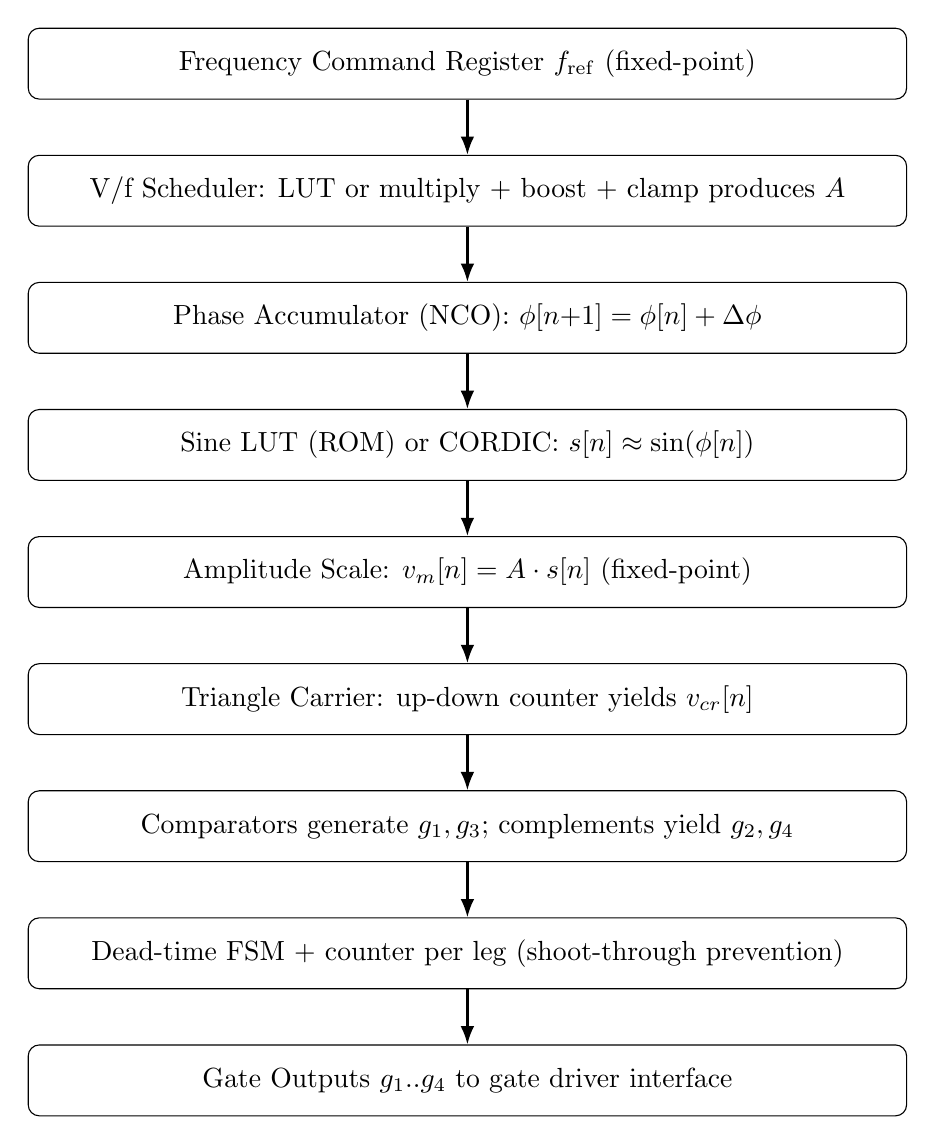
\begin{tikzpicture}[
block/.style={draw, rounded corners, minimum width=0.92\linewidth, minimum height=0.9cm, align=center},
arr/.style={-Latex, thick},
node distance=7mm
]
\node[block] (f) {Frequency Command Register $f_{\mathrm{ref}}$ (fixed-point)};
\node[block, below=of f] (vf) {V/f Scheduler: LUT or multiply + boost + clamp produces $A$};
\node[block, below=of vf] (pha) {Phase Accumulator (NCO): $\phi[n{+}1]=\phi[n]+\Delta\phi$};
\node[block, below=of pha] (lut) {Sine LUT (ROM) or CORDIC: $s[n]\approx\sin(\phi[n])$};
\node[block, below=of lut] (mul) {Amplitude Scale: $v_m[n]=A\cdot s[n]$ (fixed-point)};
\node[block, below=of mul] (car) {Triangle Carrier: up-down counter yields $v_{cr}[n]$};
\node[block, below=of car] (cmp) {Comparators generate $g_1,g_3$; complements yield $g_2,g_4$};
\node[block, below=of cmp] (dt) {Dead-time FSM + counter per leg (shoot-through prevention)};
\node[block, below=of dt] (out) {Gate Outputs $g_1..g_4$ to gate driver interface};

\draw[arr] (f) -- (vf);
\draw[arr] (vf) -- (pha);
\draw[arr] (pha) -- (lut);
\draw[arr] (lut) -- (mul);
\draw[arr] (mul) -- (car);
\draw[arr] (car) -- (cmp);
\draw[arr] (cmp) -- (dt);
\draw[arr] (dt) -- (out);
\end{tikzpicture}
\caption{Synthesizable RTL datapath for bipolar SPWM with V/f control (vertical layout).}
\label{fig:rtl}
\end{figure}

\subsection{Dead-time waveform evidence}
Your output folder currently does not contain \texttt{deadtime\_timing.png}. This report therefore includes it conditionally. When the plot exists under \texttt{../out/report/analysis/}, it will be embedded automatically; otherwise a placeholder is shown and the document still compiles.

\begin{figure}[H]
\centering
\IncludeOrPlaceholder{../out/report/analysis/deadtime_timing.png}{0.98\linewidth}
\caption{Dead-time timing evidence (non-overlap interval) derived from gate waveform transitions.}
\label{fig:deadtime}
\end{figure}

\subsection{Area, timing, and bit-width planning}
\begin{table}[H]
\centering
\begin{tabular}{@{}lccc@{}}
\toprule
\textbf{Signal} & \textbf{Typical bits} & \textbf{Format} & \textbf{Primary impact} \\
\midrule
Phase $\phi$ & 24--32 & unsigned & frequency resolution, jitter \\
Sine $s$ & 12--16 & signed $Q1.(N-1)$ & harmonic floor, LUT error \\
Amplitude $A$ & 10--14 & unsigned $Q1.(N-1)$ & V/f slope quantization \\
Carrier $v_{cr}$ & 12--16 & signed & PWM resolution, sideband shaping \\
Dead-time counter & 8--16 & unsigned & safety margin granularity \\
\bottomrule
\end{tabular}
\caption{Fixed-point sizing guidance for a synthesizable bipolar SPWM modulator.}
\label{tab:bitwidth}
\end{table}

% ============================================================
\section{Applications}

The experimentally validated bipolar SPWM with V/f control, dead-time insertion, and harmonic analysis demonstrated in this work directly maps to several high-impact power electronics and motor-drive applications. This section contextualizes the obtained waveforms, spectra, and sweep results within real deployment scenarios.

\subsection{Induction motor control (scalar V/f drive)}

Induction motors remain the most widely deployed industrial actuators due to robustness and low cost. Scalar V/f control is commonly used where precise torque control is not required.

\textbf{Relevance of results:}
\begin{itemize}
  \item The measured linear fundamental amplitude vs frequency sweep validates constant air-gap flux operation.
  \item Low-frequency operation (2--10 Hz) demonstrates stable modulation without loss of fundamental tracking.
  \item Harmonic spectra confirm dominant carrier-sideband placement, simplifying motor-side filtering.
\end{itemize}

\begin{figure}[H]
\centering
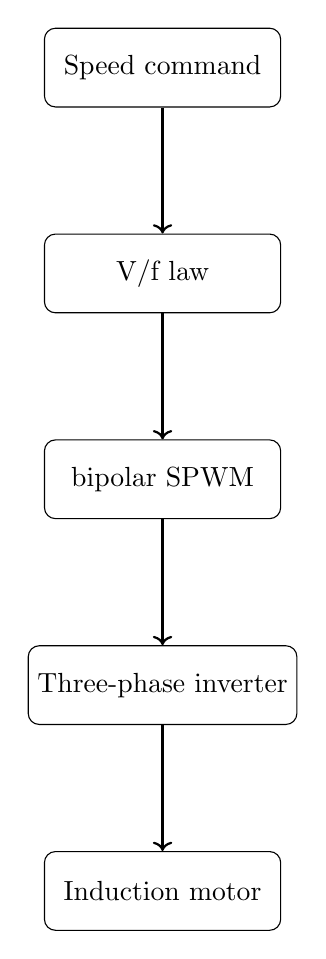
\begin{tikzpicture}[
  block/.style={draw, rectangle, rounded corners, minimum width=3cm, minimum height=1cm},
  arr/.style={->, thick},
  node distance=1.6cm
]
\node[block] (cmd) {Speed command};
\node[block, below=of cmd] (vf) {V/f law};
\node[block, below=of vf] (pwm) {bipolar SPWM};
\node[block, below=of pwm] (inv) {Three-phase inverter};
\node[block, below=of inv] (im) {Induction motor};

\draw[arr] (cmd) -- (vf);
\draw[arr] (vf) -- (pwm);
\draw[arr] (pwm) -- (inv);
\draw[arr] (inv) -- (im);
\end{tikzpicture}
\caption{Scalar V/f induction motor drive using bipolar SPWM.}
\end{figure}

This architecture corresponds directly to the measured waveforms and V/f sweep results presented earlier.

\subsection{Electric vehicle motor drives}

Electric vehicles employ high-efficiency inverters driving PMSM or induction motors under wide speed ranges.

\textbf{Relevance of results:}
\begin{itemize}
  \item bipolar SPWM reduces switching loss relative to bipolar schemes.
  \item Dead-time waveform evidence demonstrates safe high-frequency switching without shoot-through.
  \item Spectral results enable predictable EMI and acoustic noise behavior.
\end{itemize}

Although field-oriented control (FOC) is used in production EVs, the presented modulator and dead-time stage form the \emph{inner switching layer} even in vector-controlled systems.

\begin{figure}[H]
\centering
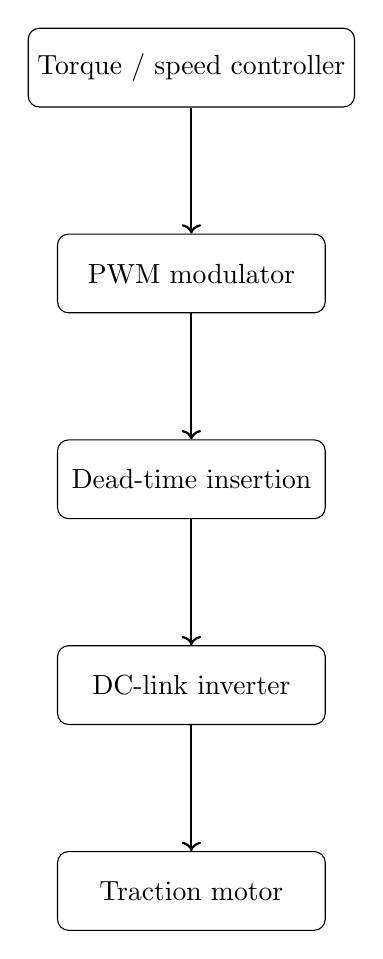
\begin{tikzpicture}[
  block/.style={draw, rectangle, rounded corners, minimum width=3.4cm, minimum height=1cm},
  arr/.style={->, thick},
  node distance=1.6cm
]
\node[block] (ctrl) {Torque / speed controller};
\node[block, below=of ctrl] (mod) {PWM modulator};
\node[block, below=of mod] (dt) {Dead-time insertion};
\node[block, below=of dt] (inv) {DC-link inverter};
\node[block, below=of inv] (mot) {Traction motor};

\draw[arr] (ctrl) -- (mod);
\draw[arr] (mod) -- (dt);
\draw[arr] (dt) -- (inv);
\draw[arr] (inv) -- (mot);
\end{tikzpicture}
\caption{EV traction inverter switching chain highlighting PWM and dead-time stages.}
\end{figure}

\subsection{Grid-connected inverter systems}

Single- and three-phase inverters are central to renewable energy integration and distributed generation.

\textbf{Relevance of results:}
\begin{itemize}
  \item FFT spectra quantify harmonic injection into the grid.
  \item Fundamental tracking validates modulation linearity under frequency variation.
  \item Switching activity sweep enables inverter loss estimation.
\end{itemize}

\begin{figure}[H]
\centering
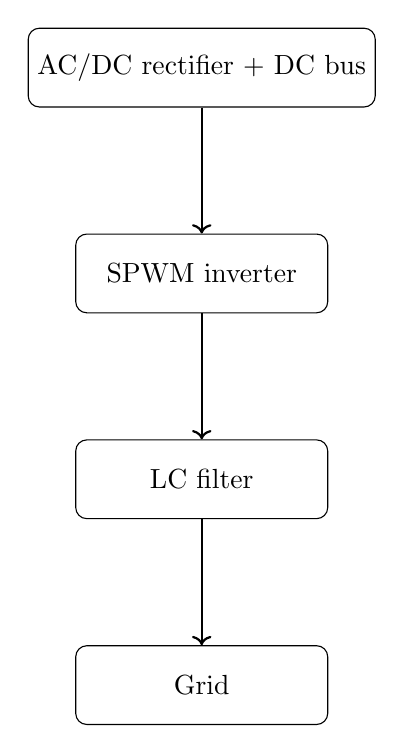
\begin{tikzpicture}[
  block/.style={draw, rectangle, rounded corners, minimum width=3.2cm, minimum height=1cm},
  arr/.style={->, thick},
  node distance=1.6cm
]
\node[block] (dc) {AC/DC rectifier + DC bus};
\node[block, below=of dc] (inv) {SPWM inverter};
\node[block, below=of inv] (lc) {LC filter};
\node[block, below=of lc] (grid) {Grid};

\draw[arr] (dc) -- (inv);
\draw[arr] (inv) -- (lc);
\draw[arr] (lc) -- (grid);
\end{tikzpicture}
\caption{Grid-tied inverter using bipolar SPWM.}
\end{figure}

The measured harmonic distribution directly informs filter design and grid-code compliance.

\subsection{Active harmonic filtering}

Active power filters inject compensating currents to cancel harmonic distortion in industrial power systems.

\textbf{Relevance of results:}
\begin{itemize}
  \item Harmonic magnitude plots identify dominant orders requiring compensation.
  \item High carrier-to-fundamental ratio enables precise current shaping.
  \item Dead-time control preserves accuracy at high switching frequencies.
\end{itemize}

\begin{figure}[H]
\centering
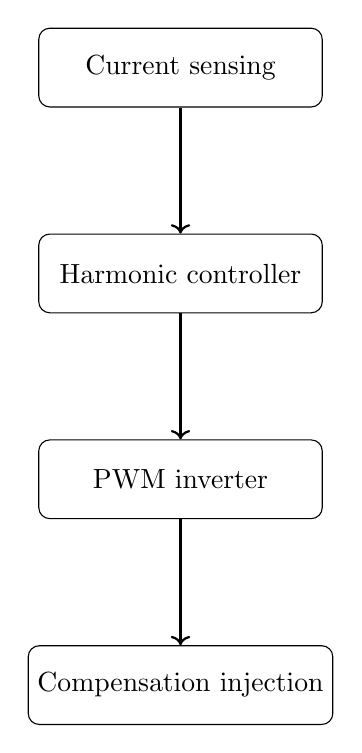
\begin{tikzpicture}[
  block/.style={draw, rectangle, rounded corners, minimum width=3.6cm, minimum height=1cm},
  arr/.style={->, thick},
  node distance=1.6cm
]
\node[block] (sense) {Current sensing};
\node[block, below=of sense] (ctrl) {Harmonic controller};
\node[block, below=of ctrl] (pwm) {PWM inverter};
\node[block, below=of pwm] (inj) {Compensation injection};

\draw[arr] (sense) -- (ctrl);
\draw[arr] (ctrl) -- (pwm);
\draw[arr] (pwm) -- (inj);
\end{tikzpicture}
\caption{Active harmonic filter based on PWM inverter.}
\end{figure}

The presented Fourier analysis and THD trends provide quantitative grounding for filter effectiveness.

% ============================================================
\section{Conclusion}
This report demonstrates bipolar SPWM with scalar V/f control using time-domain, spectral, Fourier-series, and sweep-level evidence. The harmonic structure and trends support quality-versus-stress discussion using distortion and switching proxies. A synthesizable RTL architecture is provided with explicit fixed-point definitions, carrier frequency relations, and dead-time insertion as a safety-critical FSM. This establishes a VLSI-credible foundation for implementing a digital VFD modulator in ASIC or FPGA.

\end{document}
